\documentclass{article} % for short documents
%\documentclass{report} % for longer documents


%% Defining the language for the document
\usepackage[english]{babel}
\usepackage[english]{isodate}

\usepackage{imta_core}
\usepackage{imta_extra}
\usepackage{epigraph}
\usepackage{graphicx}
\usepackage{wrapfig}
\usepackage{alertmessage}
\usepackage{hyperref}


%% Addtionnal packages can be loaded here
% \usepackage{biblatex} % for a complete and flexible bibliography


\cleanlookdateon % formats date according to the loaded language from now on

%% General informations
\author{Alexandre Allani\\
	Axel Durand\\
	Adrien Clotteau\\
	Mathieu Roy\\ 
	Matthieu Bachelot}
%\imtaAuthorShort{<author's initials>}
%\imtaSuperviser{<superviser>}
\date{\textbf{\noexpand\today}}% automatically print today's date, can be redefined using \date{<date>}
\title{Projet Statistique groupe 3}
\subtitle{La culture cinématographique}
%\imtaVersion{<version>}

%Add extra other companies' logo
%If needed, options can be passed to the underlying \includegraphics by calling \imtaAddPartnerLogo[<options>]{<path>}
%\imtaAddPartnerLogo{<logo_path>}


\imtaSetIMTStyle % Sets font and headers/footers according to the IMT Atlantue style guidelines


%%%%%%%%%%%%%%%%%%%%%%%%%%%%%%% 
%%%%%%%%%% BEGINNING %%%%%%%%%% 
\begin{document}
% front cover
\imtaMaketitlepage
\tableofcontents
\newpage
\epigraph{\large“Les cons ça ose tout, c’est même à ça qu’on les reconnait.”}{\textit{Les tontons flingueurs\\ Michel Audiard}}
\section{Contexte}
Le choix de thème de notre sondage s’est porté sur le cinéma pour deux raisons majeures : 
\begin{itemize}
	\vspace{-0.2cm}
	\setlength\itemsep{0.0cm}
	\item Nous cherchions un thème qui intéresse les sondés pour recueillir les réponses de la part d’un maximum de personnes et ainsi pouvoir faire des statistiques sans contraintes de taille d’échantillon.
	\item Nous cherchions un thème qui nous parlait à tous, qui aurait été amusant à réaliser et dont les résultats nous auraient intéressés.
\end{itemize}
Le premier point évoqué a été très important dans l’élaboration de notre questionnaire. Nous avons voulu le réaliser de manière originale, attractive et agréable à compléter afin de capter et de garder jusqu’au bout autant de sondés que possible. 
\subsection{La création du questionnaire }
Le questionnaire a été réalisé en 3 parties.
\begin{enumerate}
	\vspace{-0.2cm}
	\setlength\itemsep{0.0cm}
	\item Le recueil des informations personnelles du sondé :
	\begin{enumerate}
		\item Âge(Nombre)
		\item Sexe (homme/femme)
		\item Pays d’origine (Choix dans la liste des pays)
		\item Avez-vous étudié à IMT Atlantique (anciennement Telecom Bretagne) ? (Oui/Non)
		\item Pensez-vous reconnaître plus un film à ses répliques ou à sa musique ? (Musique/Répliques)
	\end{enumerate}
	\item Un blind test audio et visuel sur 5 films estimés comme majeurs dans l’univers cinématographique (Star Wars, le Seigneur des Anneaux, Titanic, le Roi Lion et Terminator). Par son côté ludique, celui-ci augmente l’intérêt des sondés et les motive à aller jusqu’au bout du questionnaire. Ceux-ci doivent reconnaître une réplique et une musique tirées des 5 films précédemment cités. Les dix tests (5 films et 5 musiques) sont réalisés dans un ordre que nous avons choisi pour éviter que la musique et la réplique d’un même film ne se suivent dans le sondage. Les extraits musicaux durent 20 secondes et peuvent être répétés. Pour chaque réplique et musique, les questions suivantes sont posées.
	\begin{enumerate}
		\item Connaissez-vous la référence ? (Oui/Non)
		\item (Si oui) Dans quel film l’avez vous entendu ? (Nom à marquer)
	\end{enumerate}
	\item Un sondage après révélation des films. Les cinq films sont présentés avec leurs affiches. En dessous de chaque affiche, le sondé doit répondre aux questions suivantes :
	\begin{enumerate}
		\item Combien de fois avez-vous vu ce film ? (0 fois/1 fois/2-5 fois/Plus de 5 fois)
		\item (Si plus d’une fois) À quel âge avez-vous vu ce film pour la première fois ? (0-10 ans/11-20 ans/Plus de 20 ans)
	\end{enumerate}
	\item Un notation de la part du sondé des caractéristiques qu’il juge essentielles pour qu’un film soit mémorable. Six caractéristiques sont données :
	\begin{enumerate}
		\item Répliques
		\item Musique
		\item Qualité de l’histoire
		\item Revoir un film plusieurs fois sans se lasser
		\item L’avoir vu enfant
		\item Porteur d’émotion\\Pour chaque caractéristique, le sondé devra choisir entre : D’accord/Plutôt d’accord/Neutre/Plutôt pas d’accord/Pas d’accord.
	\end{enumerate}
\end{enumerate}
Les 5 films que nous avons sélectionnés correspondent à des films de différents genres destinés à différents publics et sortis lors de différentes décennies (Star Wars : 1977, le Seigneur des Anneaux : 2001, Titanic : 1997, le Roi Lion : 1994 et Terminator : 1984). Cependant, ils correspondent à des films cultes selon les critères de notre génération et peuvent ne pas être considérés comme tels par les autres.
\subsection{ Le choix d'échantillonnage }
N’ayant pas un large choix de sondeurs (étudiants d’IMT Atlantique, familles etc …), nous avons fait le choix de ne pas échantillonner nos sondés pour avoir le plus de réponses possibles. De plus, notre thème est censé devoir toucher tout type de population. Il a été donc important, dans notre sondage, de demander les caractéristiques des sondés (âge, nationalité, étudiant d’IMT).

\subsection{Étude de l’échantillon}
Nous avons obtenu 388 réponses au sondage. 86 d’entre elles n’étaient pas complètes. Deux autres données étaient obsolètes, ce qui ramène le nombre de réponses traitées à 300. Parmi ces données, deux individus ont donné des âges incohérents, ils ne seront donc pas étudiés pour les statistiques par rapport à l’âge.\\
\begin{figure}[!h]
	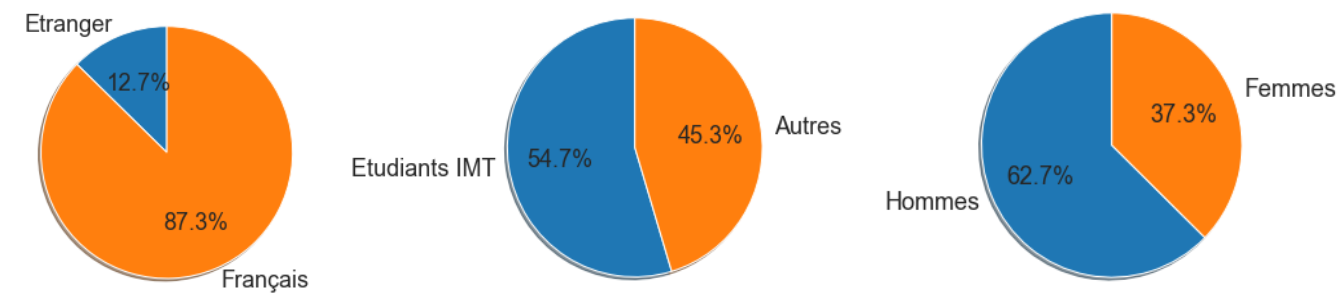
\includegraphics[keepaspectratio,scale=0.6]{piechart.png}
	\caption{Caractéristiques des sondés}
\end{figure}~\\

\begin{wrapfigure}[11]{L}{100mm}
	\centering
	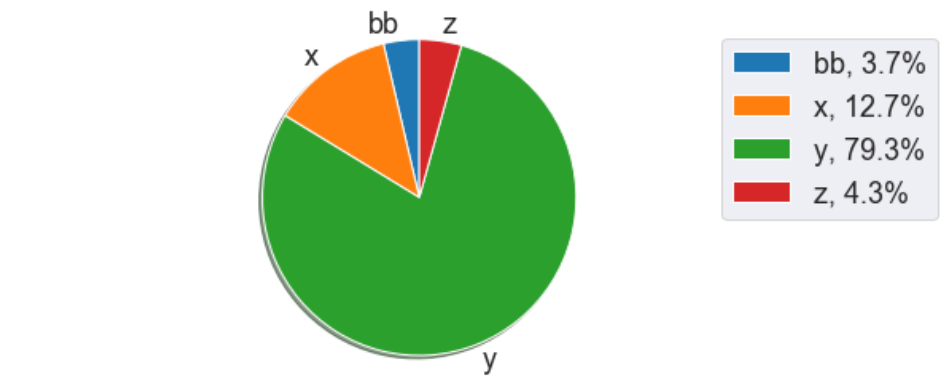
\includegraphics[keepaspectratio = true,scale=0.38]{piechar2}
	\caption{Générations auxquelles appartiennent les sondés}
\end{wrapfigure}

On peut remarquer une grande proportion d’étudiants IMT, de Français et d’hommes dans nos échantillons. De plus, les réponses à la question “Pensez-vous reconnaître plus un film par ses musiques ou par ses répliques ?” sont équitablement réparties (52,3\% pour les répliques contre 47,7\% pour les musiques).\\
On peut aussi remarquer une grande proportion d’individus de la génération Y (18-38 ans) qui correspond à la tranche d’âge des étudiants d’IMT Atlantique et un faible nombre de baby-boomers (plus de 54 ans) et de générations Z (moins de 18 ans).
\newpage
\section{Analyse statistiques de l'échantillon: les hypothèses et leur vérification}
\alertinfo{Vous pouvez retrouver une version plus détaillé de l'analyse des résultats (avec le code) en cliquant sur le lien suivant : \url{https://github.com/Syndorik/ProjetStats/blob/master/Projet\%20Stats.html}. Il faut télécharger le fichier afin de pouvoir visualiser les graphiques}
Dans la partie qui suit, nous allons énumérer les différentes hypothèses que nous avons posées, ainsi que l’analyse statistique faite pour les valider (ou invalider).\\
Les lois de distribution de nos variables ne sont pas normalement distribuées et sont discrètes. Cependant, par le théorème de centrale limite, vu que notre échantillon n est grand (n = 300), la distribution des moyennes tend vers une loi normale. On utilise ce théorème pour toutes nos hypothèses.
\subsection{Hypothèse 1}
H0 = Les sondés reconnaissent autant un film par sa musique que par sa réplique.
\begin{itemize}
	\vspace{-0.2cm}
	\setlength\itemsep{0.0cm}
	\item $H0: \ \mu{musique} = \mu{réplique}$
	\item $H1: \ \mu{musique} \ne \mu{réplique}$
\end{itemize}
Le but ici est, comme l’indique l’intitulé de l’hypothèse, de comparer les taux de bonnes réponses au blind test, pour les musiques et pour les répliques.
\subsubsection{Visualisation}
\begin{figure}[!h]
	\centering
	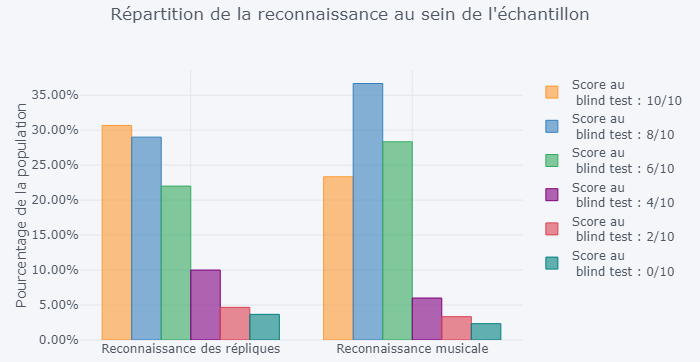
\includegraphics[keepaspectratio,scale=0.9]{h1.png}
	\caption{ Pourcentage de reconnaissance des musiques et répliques}
\end{figure}~\\
La répartition correspond à nos attentes. Nous cherchions des films que l'ensemble des sondés pouvaient connaître, mais qui n'étaient pas non plus reconnus par tout le monde. On peut remarquer qu'il y a plus de personnes ayant reconnu l'ensemble des répliques que des musiques. Cependant il y a plus de gens ayant reconnus au moins 3 musique que de gens ayant reconnu au moins 3 répliques.
\subsubsection{Application du test}
En regardant notre hypothèse, avec l’hypothèse nulle et l’hypothèse alternative, on remarque que l’on peut utiliser ici un test de Student. Par ailleurs les données sont appariées (la musique et la réplique sont associées pour une même personnes). 
De plus, les échantillons sont bien indépendants.\\

La moyenne de reconnaissance des répliques est de 0.73 et la moyenne de reconnaissance des musiques est de 0.72.Immédiatement, en regardant le résultat, on peut s’attendre à ce que le test confirme l’hypothèse nulle.\\
Après application du test, nous obtenons les valeurs suivantes : $pvalue = 0.5817$, $t = 0.5514$. Donc ${pvalue>0.05}$. De plus, l'intervalle de confiance des différences de moyenne est de : [-0.05,0.03]. La différence des moyennes observées appartenant à l'échantillon est en accord avec la pvalue calculée

\alertsuccess{
	 On peut conclure que les sondés reconnaissent autant un film par sa musique que par sa réplique.
}

\subsection{ Hypothèses 2.1 et 2.2}
H2.1 : les hommes reconnaissent plus les films par la réplique que les femmes.
De nouveau nous faisons un test de Student, avec pour hypothèses:
\begin{itemize}
	\vspace{-0.2cm}
	\setlength\itemsep{0.0cm}
	\item $H_0: \ \mu_{homme\_rep} = \mu{femme\_rep}$
	\item $H_a: \ \mu_{homme\_rep} \ne \mu{femme\_rep}$
\end{itemize}
H2.2 : Les femmes reconnaissent plus les films par les musiques que les hommes.
Test de Student, avec pour hypothèses:
\begin{itemize}
	\vspace{-0.2cm}
	\setlength\itemsep{0.0cm}
	\item $H_0: \ \mu_{homme\_mus} = \mu{femme\_mus}$
	\item $H_a: \ \mu_{homme\_mus} \ne \mu{femme\_mus}$
\end{itemize}
Le but ici est de comparer la reconnaissance des films par les hommes et les femmes.
Pour les deux hypothèses, nous allons appliquer le test de Student.
\subsubsection{Visualisation}
\begin{figure}[!hbt]
	\centering
	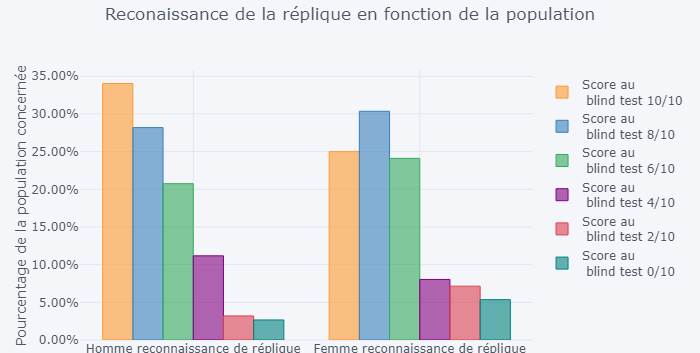
\includegraphics[keepaspectratio,scale=0.9]{h21.png}
	\caption{ Pourcentage de reconnaissance des répliques pour les hommes et les femmes}
\end{figure}~\\
\begin{figure}[!hbt]
	\centering
	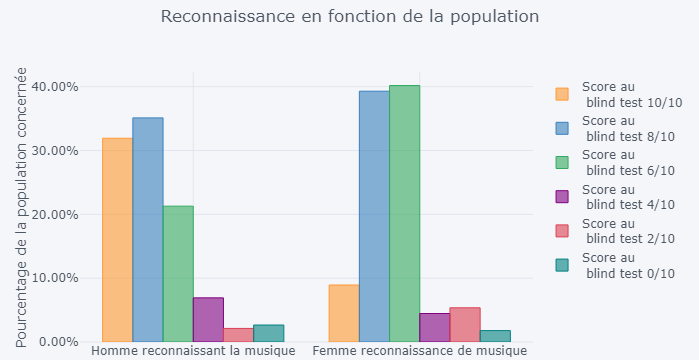
\includegraphics[keepaspectratio,scale=0.9]{h22.png}
	\caption{ Pourcentage de reconnaissance des musiques pour les hommes et les femmes}
\end{figure}~\\
La distribution entre les hommes et les femmes est assez différente. En particulier les hommes ont l'air de reconnaître mieux à la réplique contrairement aux femmes. Pareillement, les hommes ont l'air de reconnaître mieux la musique que les femmes.
\subsubsection{ Application des test}

\paragraph{Test hypothèse 2.1:\\} Les hommes reconnaissent plus les films par la réplique que les femmes \\
Après application du test, nous obtenons les valeurs suivantes : $pvalue = 0.070$, $t = 1.814$. Donc ${pvalue>0.05}$. De plus, l'intervalle de confiance des différences de moyenne est de : [-0.12,0.01].
\alertsuccess{On ne peut pas affirmer l'hypothèse nulle. En effet, la p-value qu'on obtient après le test de student est de 0.07. Cependant, la pvalue étant très proche de 0.05, utilisé communément en statistique pour rejeter l'hypothèse, nous pouvons en déduire qu'il y a de forte présomption contre l'hypothèse.}
\paragraph{Test hypothèse 2.2:\\} Les femmes reconnaissent plus les films par la musique que les hommes.
Après application du test, nous obtenons les valeurs suivantes : $pvalue = 0.001$, $t = 3.219$. Donc ${pvalue<0.05}$. De plus, l'intervalle de confiance des différences de moyenne est de : [-0.14,-0.04].
\alertsuccess{On peut rejeter l’hypothèse nulle via la pvalue. }
\subsubsection{Conclusion des tests}
Les hommes reconnaissent mieux les répliques et les musiques que les femmes. Ce résultat pouvait être anticipable. En effet, comme nous l’expliquerons dans les biais du sondage un peu plus tard, dans notre groupe nous sommes 6 hommes, et donc notre choix de film a été influencé, avec plus de chance d’être réussi par d’autres hommes.
\subsection{Hypothèses 3.1 et 3.2}
Nous comparons ici les femmes ayant répondu différemment à la question préliminaire “Pensez-vous reconnaitre un film plus à ses répliques ou à sa musique?”. L’intérêt de cette hypothèse est de voir si les femmes savent comment elles vont reconnaître les films.\\
Pour les deux hypothèses, nous appliquons un test de Student.\\

H3.1 : Les femmes pensant reconnaître les films plus par la musique reconnaissent autant la musique que celles qui pensent reconnaître les films par la réplique.
\begin{itemize}
	\item $H_0: \ \mu_{femme\_recmus} = \mu_{femme\_recrep}$
	\item $H_a: \ \mu_{femme\_recmus} \ne \mu_{femme\_recrep}$
\end{itemize}

Ici $\mu_{femme\_recmus}$ représente la moyenne des réponses (sur la musique) des femmes pensant reconnaître la musique.  $\mu_{femme\_recrep}$ représente la moyenne des réponses (sur la musique) des femmes pensant reconnaître la réplique.
\subsubsection{Hypothèse 3.1 :}
\paragraph{ Application des test\\}
La moyenne de femme pensant reconnaître la musique et qui reconnaissent la musique est de 0.68. La moyenne de femme pensant reconnaître la réplique et qui reconnaissent la musique est de 0.67.\\
Après application du test, nous obtenons les valeurs suivantes : $pvalue =  0.7452$, $t = 0.3257$. Donc ${pvalue>0.05}$. De plus, l'intervalle de confiance des différences de moyenne est de : [-0.09,0.06]. La différence des moyennes observées appartenant à l'échantillon est en accord avec la pvalue calculée.
\alertsuccess{Avec cette valeur de pvalue, nous pouvons affirmer l’hypothèse nulle.}
\alertwarning{Dans notre questionnaire nous n'avons pas mis de case "Je reconnais un film par la musique et par les répliques". Ainsi une personne ayant tout reconnu en film et en réplique ferait plutôt parti de cette population. Cela biaise un peu le résultat précédent. }
\alertwarning{On applique de nouveau un test de Student mais cette fois-ci sans prendre en compte celles qui ont fait un 100\% au blind test afin d'éliminer ce biais}

La moyenne de femme pensant reconnaître la musique et qui reconnaissent la musique est de 0.66. La moyenne de femme pensant reconnaître la réplique et reconnaissant la musique est de 0.65.\\
Après application du test, nous obtenons les valeurs suivantes : $pvalue =   0.7657$, $t =  0.2986$. Donc ${pvalue>0.05}$. De plus, l'intervalle de confiance des différences de moyenne est de : [-0.09,0.06]. La différence des moyennes observées appartenant à l'échantillon est en accord avec la pvalue calculée.
\alertsuccess{Avec cette valeur de pvalue, nous devons toujours confirmer l’hypothèse nulle (le biais est toujours présent). Ainsi, avoir choisi “musique” ou “réplique” dans la question préliminaire n’implique pas une différenciation de bonnes réponses sur la musique, pour les femmes.}
\newpage
\subsubsection{Hypothèse 3.2:}
H3.2 : Les femmes pensant reconnaître les films plus par la réplique reconnaissent autant la réplique que celles qui pensent reconnaître les films par la musique.
\begin{itemize}
	\item $H_0: \ \mu_{femme\_recmus} = \mu_{femme\_recrep}$
	\item $H_a: \ \mu_{femme\_recmus} \ne \mu_{femme\_recrep}$
\end{itemize}

Ici $\mu_{femme\_recmus}$ représente la moyenne des réponses (sur la réplique) des femmes pensant reconnaître la musique. $\mu_{femme\_recrep}$ représente la moyenne des réponses (sur la réplique) des femmes pensant reconnaître la réplique.
\paragraph{ Application des test\\}
On choisit immédiatement de ne pas prendre en compte les femmes ayant répondu bon à 100\% au blind test.\\
La moyenne de femme pensant reconnaître la musique et reconnaissant les répliques est de 0.63. La moyenne de femme pensant reconnaître la réplique et reconnaissant les répliques est de 0.71.\\
Après application du test, nous obtenons les valeurs suivantes : $pvalue = 0.1456$, $t = -1.466$. Donc ${pvalue>0.05}$. De plus, l'intervalle de confiance des différences de moyenne est de : [-0.03,0.19].
\alertsuccess{Après application du test, nous devons accepter l'hypothèse nulle. La pvalue, bien que plus faible qu’au test précédent, reste supérieur à 0.05.}
\subsubsection{Conclusion des tests}
Avec ces tests, nous pouvons affirmer que la réponse à la question préliminaire est très peu pertinente pour les femmes, dans ce sondage. Le fait que nos films soient peu nombreux et plutôt “simple” à reconnaître empêche un clivage marquant avec la question préliminaire.

\subsection{Hypothèses 4.1 et 4.2}
Nous comparons ici les hommes ayant répondu différemment à la question préliminaire “Pensez-vous reconnaitre un film plus à ses répliques ou à sa musique?”. L’intérêt de cette hypothèse est de voir si les hommes savent comment ils vont reconnaître les films.
Pour les deux hypothèses, nous appliquons un test de Student.
\alertinfo{En continuation avec les tests sur les femmes, nous choisissons d’exclure les hommes ayant eu 100\% au blind test.}
\subsubsection{Hypothèse 4.1}
H4.1 : Les hommes pensant reconnaître les films plus par la musique reconnaissent autant la musique que ceux qui pensent reconnaître les films par la réplique.
\begin{itemize}
	\item $H_0: \mu_{homme\_recmus} = \mu_{homme\_recrep} $
	\item $H_a: \mu_{homme\_recmus} = \mu_{homme\_recrep} $
\end{itemize}

Ici $\mu_{homme\_recmus}$ représente la moyenne des réponses (sur la musique) des hommes pensant reconnaître la musique. $\mu_{homme\_recrep}$ représente la moyenne des réponses (sur la musique) des hommes pensant reconnaître la réplique.
\paragraph{Application du test\\}
La moyenne des hommes pensant reconnaître la musique et reconnaissant la musique est de 0.72. La moyenne des hommes pensant reconnaître la réplique et reconnaissant la musique est de 0.67.\\
Après application du test, nous obtenons les valeurs suivantes : $pvalue = 0.2054$, $t = 1.271$. Donc ${pvalue<0.05}$. De plus, l'intervalle de confiance des différences de moyenne est de : [-0.12,0.03].
\alertsuccess{Avec cette valeur de pvalue, nous pouvons affirmer l’hypothèse nulle.}
\subsubsection{Hypothèse 4.2}
H4.2 : Les hommes pensant reconnaître les films plus par la réplique reconnaissent autant la réplique que ceux qui pensent reconnaître les films par la musique.
\begin{itemize}
	\item $H_0: \mu_{homme\_recmus} = \mu_{homme\_recrep} $
	\item $H_a: \mu_{homme\_recmus} = \mu_{homme\_recrep} $
\end{itemize}
Ici $\mu_{homme\_recmus}$ représente la moyenne des réponses (sur la réplique) des hommes pensant reconnaître la musique.  $\mu_{homme\_recrep}$ représente la moyenne des réponses (sur la réplique) des hommes pensant reconnaître la réplique.
\paragraph{ Application des test}
La moyenne des hommes pensant reconnaître la musique et reconnaissant la réplique est de 0.68.
La moyenne des hommes pensant reconnaître la réplique et reconnaissant la réplique est de 0.67.\\
Après application du test, nous obtenons les valeurs suivantes :$pvalue = 0.8612$, $t = 0.1751$. Donc ${pvalue>0.05}$. De plus, l'intervalle de confiance des différences de moyenne est de :  [-0.09,0.07].
\alertsuccess{Avec cette valeur de pvalue, nous pouvons affirmer l’hypothèse nulle. }
\subsubsection{Conclusion}
Avec ces tests, nous pouvons affirmer que la réponse à la question préliminaire est très peu pertinente pour les hommes aussi, dans ce sondage. 

\subsection{ Hypothèse 5}
H5 : Les français reconnaissent les films proposés autant que les autres nationalités.
\begin{itemize}
	\item $H_0: \ \mu_{nationalité} = \mu_{francais}$
	\item $H_a: \ \mu_{nationalité} \ne \mu_{francais}$
\end{itemize}
Nous appliquons de nouveau le test de Student.
\newpage
\subsubsection{Visualisation}
\begin{figure}[!h]
	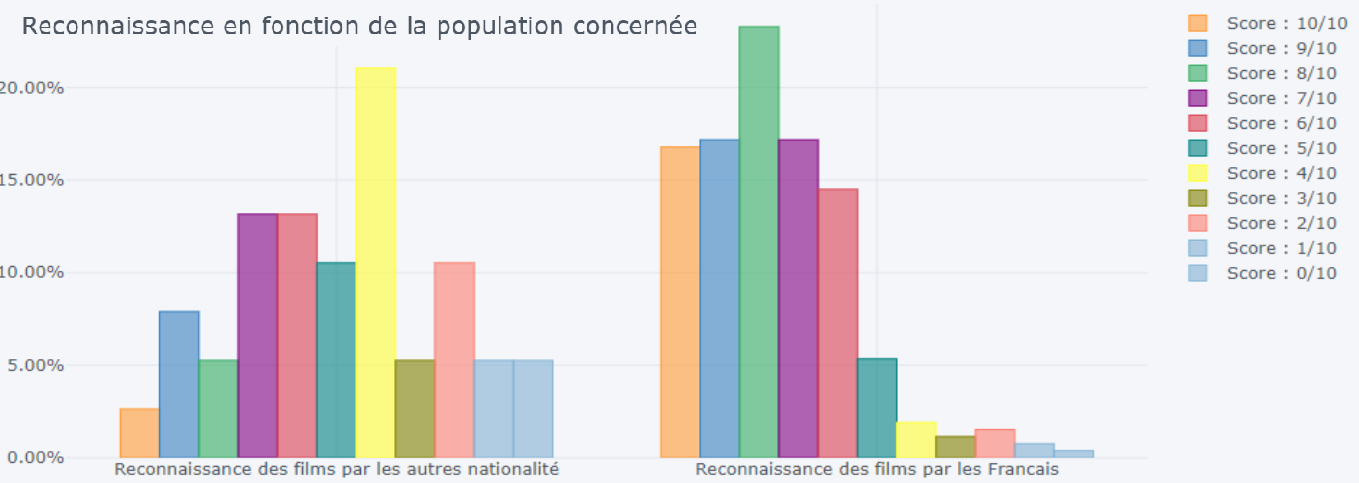
\includegraphics[keepaspectratio,scale=0.6]{h5.png}
	\caption{Score au blind test en fonction de la nationalité}
\end{figure}~\\
Ce graphe nous permet immédiatement de prévoir le résultat flagrant du test, c’est à dire la validation de l’hypothèse alternative.
\subsubsection{ Application des test}
La moyenne de reconnaissance de film par les français est de 0.76 et la moyenne de reconnaissance de film par les autres autres nationalités est de 0.49.\\
Après application du test, nous obtenons les valeurs suivantes : $pvalue = 2.3920e^{-13}$, $t = 7.674$. Donc ${pvalue<0.05}$. De plus, l'intervalle de confiance des différences de moyenne est de : [-0.36,-0.18].
\alertsuccess{Après application du test, on peut rejeter l'hypothèse nulle. En effet la pvalue est presque nulle donc inférieure à 0.05. Ainsi, nous avons la confirmation que les français on mieux répondus au blind test que les étrangers. Nous avions conscience de ce biais à la création du sondage et nous voulions voir s'il était confirmé. Cela est bien le cas}
\subsection{ Hypothèse 6}
H5.5 : Parmi les différentes générations (baby-boomers / X / Y / Z), la génération Y (née entre 1980 et 2000) a une meilleure connaissance des films qui sont proposés.
\begin{itemize}
	\item $H_0: \ \mu{babyboomer} = \mu_{X} = \mu_{Y} = \mu{Z}$
	\item $H_a$ : Il y a une différence parmi les moyennes
\end{itemize}
On va utiliser ANOVA pour confirmer ou infirmer les hypothèses. De même que pour Student, bien que nos variables prennent des valeurs discrètes et leur distribution n'est pas normale, on peut appliquer l'ANOVA grâce à la taille de l'échantillon.
\newpage
\subsubsection{Visualisation}
\begin{figure}[!h]
	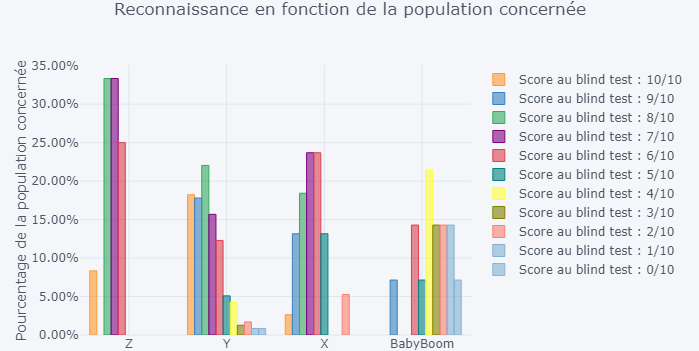
\includegraphics[keepaspectratio,scale=0.9]{h6.png}
	\caption{Score au blind test en fonction de la génération}
\end{figure}~\\
Il y a 38 personnes dans la génération X, 236 dans la génération Y, 12 dans la génération Z et 14 dans la génération BabyBoomer.\\
On remarque que la génération Y est celle qui est la plus représentée. Cela introduit un fort biais pour le test suivant car la génération Z et la génération Babyboomer sont sous-représentées. Ainsi les tests de Normalité pour les distributions de la génération Z et Babyboom peuvent être remis en cause (annulant donc la possibilité d'ANOVA).\\
\alertwarning{Nous continuons ici en supposant que l’ANOVA est possible.}
\subsubsection{ Application des test}
La moyenne de Z est de 0.73. La moyenne de Y est de 0.75. La moyenne de X est de 0.68. La moyenne de BabyBoomer est de 0.36.\\
Après application du test, nous obtenons les valeurs suivantes : $pvalue = 2.073e^{-10}$, $t = 17.36$. Donc ${pvalue<0.05}$.\\
Bien que les échantillons soient peu représentatifs de toutes les générations, le test ANOVA infirme l'hypothèse de base. En effet la pvalue est bien inférieure à 0.05. Donc les moyennes sont différentes. On remarque que la moyenne des BabyBoomer est bien en deçà du reste.
\alertwarning{Pour rappel l'échantillon des babyboomers est très peu représentatif.}
On refait une ANOVA pour comparer les génération X, Y et Z.
Après application du test, nous obtenons les valeurs suivantes : $pvalue =  0.0980$, $t = 2.341$. Donc ${pvalue<0.05}$.\\
\alertsuccess{Ici la p-value est de 0.10, nous ne pouvons rejeter l'hypothèse nulle. Cependant il y a tout de même de fortes présomptions contre le modèle. Il est intéressant de noter que, les trois génération ont été marquées par ces films. Ils sont donc inter-générationnels, ce nous voulions puisque c’est un critère des films cultes.}
Pour rappel, les conclusions tirées de ce test sont à relativiser car l'ANOVA ici est hautement faussé par la taille très faible de l'échantillon.
\subsection{Hypothèse 7}
Les personnes n’ayant pas vu le film reconnaissent aussi bien que celles qui l’ont vu.
\begin{itemize}
	\item $H_0 : \mu_{film\_pas\_vu\_mais\_reconnu} = \mu_{vu\_film\_et\_reconnu}$
	\item $H_a : \mu_{film\_pas\_vu\_mais\_reconnu} \ne \mu_{vu\_film\_et\_reconnu}$
\end{itemize}
L’objectif est de comparer, film par film, si les gens n’ayant pas vu ce film peuvent en connaître les répliques et musiques aussi bien que ceux qui l’ont déjà regardé.
\subsubsection{Visualisation}
\begin{figure}[!h]
	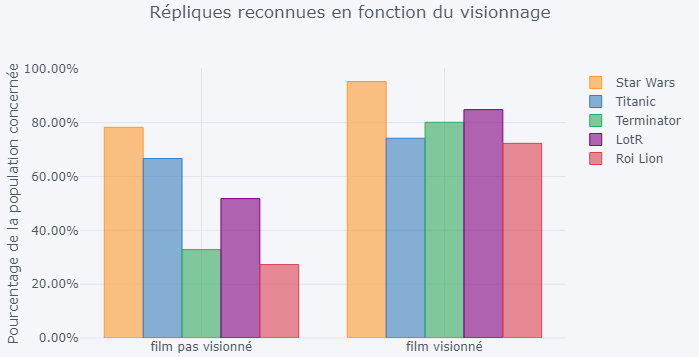
\includegraphics[keepaspectratio,scale=0.9]{h7.png}
	\caption{Reconnaissance de la musique sachant que le film a été visionné ou non}
\end{figure}~\\
\begin{figure}[!h]
	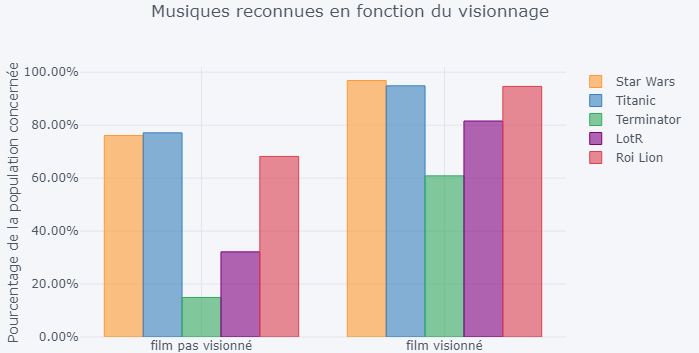
\includegraphics[keepaspectratio,scale=0.9]{h61.png}
	\caption{Reconnaissance de la réplique sachant que le film a été visionné ou non}
\end{figure}~\\
Comme prévu, tous les films semblent être mieux reconnus en répliques et musiques lorsque le film a été visionné. Cependant, cela semble varier d’un film à l’autre, nous allons le vérifier. 
\\
On peut remarquer avec ces deux graphiques, qu'en moyenne, ceux qui ont vu Terminator ont deux fois plus de chance de trouver la réponse au Blind Test que ceux qui ne l'ont pas vu. Ce film étant le moins populaire, cela nous conforte dans nos prédictions
\\
De plus, Titanic est le film le plus vu de tous les temps au box-office français et Star Wars est extrêmement populaire. Il est normal que les personnes ne les ayant pas vu en aient été fortement imprégnées par leur entourage et donc que les meilleures scores des films non visionnés soient pour ces deux films.
\\
\alertinfo{Seulement 22 personnes sur les 300 interrogées n’avaient jamais vu le Roi Lion, ce qui perturbe fortement les mesures et leur donne une grande volatilité. Nous pourrions remettre en cause la viabilité d'un test de Student. Cependant, vu le nombre de personnes n’ayant pas vu les 4 autres films, cette valeur est acceptable.}
\subsubsection{ Application des test}
Nous appliquons un test t de Student apparié pour chaque film.
\paragraph{H7.1: Les personnes n’ayant pas vu Star Wars reconnaissent aussi bien que celles qui l’ont vu.\\}
La moyenne de pourcentage de reconnaissance du film par ceux qui ne l'ont pas vu est de 0.75 et la moyenne de pourcentage de reconnaissance du film par ceux qui l'ont vu est de 0.95\\
Après application du test, nous obtenons les valeurs suivantes : $pvalue =  1.143e^{-08}$, $t = -5.872$.L'intervalle de confiance des différence de moyenne est de : [0.10,0.31].
\alertsuccess{pvalue << 5\% donc on peut rejeter l'hypothèse nulle. Les personnes n’ayant pas vu Star Wars reconnaissent moins bien que celles qui l’ont vu.} 

\paragraph{H7.2: Les personnes n’ayant pas vu le Roi Lion reconnaissent aussi bien que celles qui l’ont vu. \\}
La moyenne de pourcentage de reconnaissance du film par ceux qui ne l'ont pas vu est de 0.39 et la moyenne de pourcentage de reconnaissance du film par ceux qui l'ont vu est de 0.79\\
Après application du test, nous obtenons les valeurs suivantes : $pvalue =  1.805e^{-08}$, $t = -5.7877$.L'intervalle de confiance des différence de moyenne est de : [0.23,0.59]..
\alertsuccess{Les personnes n’ayant pas vu le Roi Lion reconnaissent moins bien que celles qui l’ont vu. } 

\paragraph{H7.3: Les personnes n’ayant pas vu Terminator reconnaissent aussi bien que celles qui l’ont vu. }
La moyenne de pourcentage de reconnaissance du film par ceux qui ne l'ont pas vu est de 0.18 et la moyenne de pourcentage de reconnaissance du film par ceux qui l'ont vu est de 0.64\\
Après application du test, nous obtenons les valeurs suivantes : $pvalue = 9.7334e^{-08}$, $t = 12.395$.L'intervalle de confiance des différence de moyenne est de : [0.40,0.54].
\alertsuccess{Les personnes n’ayant pas vu Terminator reconnaissent moins bien que celles qui l’ont vu. } 

\paragraph{H7.4: Les personnes n’ayant pas vu Titanic reconnaissent aussi bien que celles qui l’ont vu. \\}
La moyenne de pourcentage de reconnaissance du film par ceux qui ne l'ont pas vu est de 0.68 et la moyenne de pourcentage de reconnaissance du film par ceux qui l'ont vu est de 0.81\\
Après application du test, nous obtenons les valeurs suivantes : $pvalue =  0.0036$, $t = -2.9335$.L'intervalle de confiance des différence de moyenne est de : [0.03,0.25].
\alertsuccess{Les personnes n’ayant pas vu Titanic reconnaissent moins bien que celles qui l’ont vu. } 

\paragraph{H7.5: Les personnes n’ayant pas vu le Seigneur des anneaux reconnaissent aussi bien que celles qui l’ont vu.\\}
La moyenne de pourcentage de reconnaissance du film par ceux qui ne l'ont pas vu est de 0.34 et la moyenne de pourcentage de reconnaissance du film par ceux qui l'ont vu est de 0.79\\
Après application du test, nous obtenons les valeurs suivantes : $pvalue =   3.6178e^{-16}$, $t = -8.6347$.L'intervalle de confiance des différence de moyenne est de : [0.34,0.55].
\alertsuccess{Les personnes n’ayant pas vu le Seigneur des Anneaux reconnaissent moins bien que celles qui l’ont vu. } 

\subsubsection{Conclusion}
On remarque que toutes les sous-hypothèses de l'hypothèse 6 ont une p-value très faible, et bien inférieure à 0.05. Nous pouvons donc rejeter l'hypothèse nulle de toutes les hypothèses. Ainsi, comme nous pouvions nous en douter, les personnes ayant vu le film reconnaissent mieux le film lors du blind test comparé à ceux qui ne l'ont jamais visionné. 
En cohérence avec ce qui a été dit plus tôt, Terminator a bien la p-value la plus faible (E-29) et Titanic la plus élevée (0.3\%).

\subsection{Hypothèse 8}
H7: Un film vu jeune a plus d’impact sur la mémoire (reconnaissance de réplique OU musique du film au blind test) qu’un autre.
\begin{itemize}
	\item $H_0: \ \mu_{0-10} = \mu_{11-20}= \mu_{>20}$
	\item $H_a$ : Il y a une différence de moyenne
\end{itemize}
Nous essayons de voir ici si l'âge de premier visionnage a un impact sur la mémorisation d’un film.
\newpage
\subsubsection{Visualisation}

\begin{figure}[!h]
	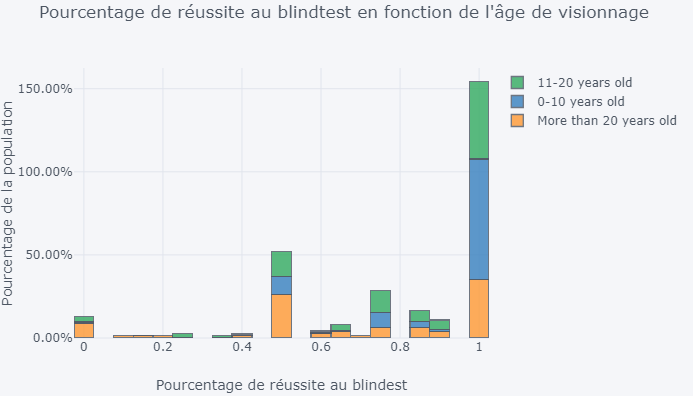
\includegraphics[keepaspectratio,scale=0.6]{h8.png}
	\caption{Pourcentage de réussite au blindtest en fonction de l'âge de visionnage}
\end{figure}~\\
On remarque qu’une tendance se dégage: pour ceux qui ont vu le film avant leur 10 ans (rectangles bleus sur le graphe), ils ont tous plus de 50\% de réussite au blind test. 
\subsubsection{ Application des test}
Il y a 77 échantillon dans la catégorie More than 20 years old\\
Il y a 212 échantillon dans la catégorie 0-10 years old\\
Il y a 268 échantillon dans la catégorie 11-20 years old\\
\alertinfo{On peut remarquer que le nombre d'échantillon est cette fois-ci suffisant pour appliquer un test ANOVA.}
La moyenne de 0-10 years old est de 0.90. La moyenne de 11-20 years old est de 0.79. La moyenne de More than 20 years old est de 0.68.\\
Après application du test, nous obtenons les valeurs suivantes : $pvalue =   7.3964e^{-11}$, $t = 24.337$.\\
En appliquant le test on remarque qu'on ne peut accepter l'hypothèse nulle car la p-value est bien inférieure à 0.05. Ainsi, au vu des moyennes calculés précédemment, on peut déjà conclure que les personnes ayant le film dans leurs 20 ans sont moins susceptible de reconnaître un film considéré dans ce sondage comme "mémorable”.
\alertinfo{Nous allons appliquer un test de student deux à deux sur les population More than 20 years old, 0-10 years old et 11-20 years old, afin de déterminer lesquels diffèrent et le possible classement que l'on peut faire.}
\begin{itemize}
	\item \textbf{Student pour 0-10 years et 11-20 years: } Après application du test, nous obtenons les valeurs suivantes : $pvalue =   1.4293e^{-6}$, $t = 4.8826$. L'intervalle de confiance des différences de moyenne est de : [-0.15,-0.06].\\
	\item \textbf{Student pour 11-20 years et more than 20 year: }Après application du test, nous obtenons les valeurs suivantes : $pvalue =   0.001$, $t = 3.1913$.L'intervalle de confiance des différences de moyenne est de : [-0.19,-0.03].\\
\end{itemize}
\alertsuccess{Les 2 tests de Student réalisés ont une p-value inférieure à 5\%. Nous rejetons donc l'hypothèse nulle pour chaque test. Ainsi, comme le laissait suggérer l'ANOVA, nous pouvons conclure que plus une personne voit un film étant jeune, plus il est mémorable pour l’individu.}

\subsection{Hypothèses 9}
Le but de cette section est de juger l’importance de certaines caractéristiques d’un film.
\begin{itemize}
	\item $H_{9.1}$ : L’histoire est importante pour qu’un film soit mémorable
	\item $H_{9.2}$: Pouvoir revoir un film plusieurs fois sans se lasser est important pour que le film soit mémorable
	\item $H_{9.3}$: Avoir vu un film enfant est important pour que ce film soit mémorable
	\item $H_{9.4}$: Le fait qu’être porteur d’émotion est important pour que ce film soit mémorable
	\item $H_{9.5}$: La musique est importante pour qu’un film soit mémorable
	\item $H_{9.6}$: Les répliques sont importantes pour qu’un film soit mémorable
\end{itemize}
Vu que les variables sont categorielles et que l'ont cherche a déterminer quel est la plus grande opinion au sein de la population, nous allons faire des tests du $\chi^1$.Les hypothèses de test sont les suivantes :
\begin{itemize}
	\item $H_0: \ p_{D'accord}=p_{Plutôt d'accord} = p_{Neutre} = p_{Plutôt pas d'accord}= p_{Pas d'accord}$ 
	\item $H_a: \ $Les proportions sont différentes
\end{itemize}
Ainsi, pour affirmer nos hypothèses écrites plus haut, nous devons invalider l’hypothèse nulle pour chaque caractéristique.

\subsubsection{Visualisation}

\begin{figure}[!h]
	\centering
	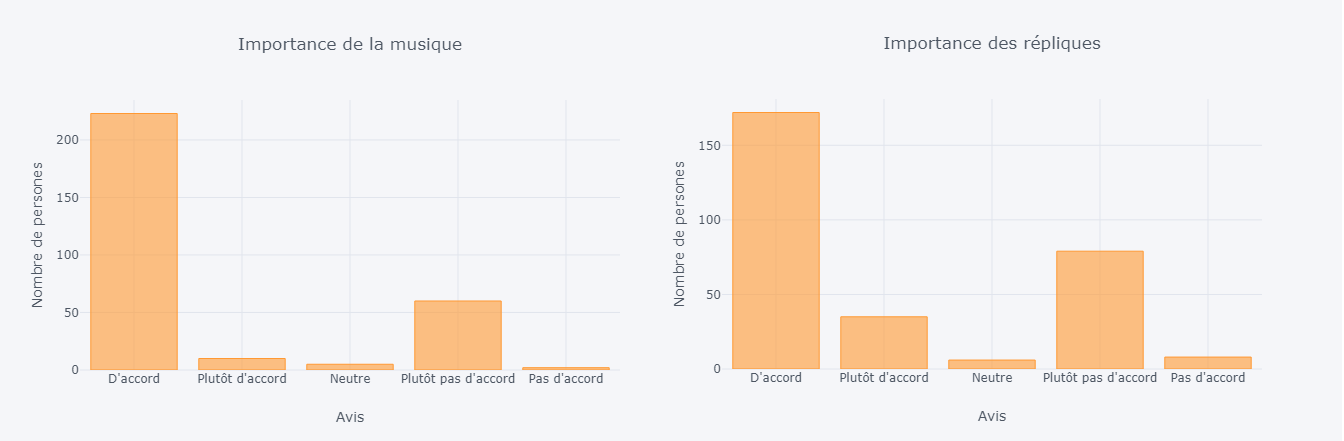
\includegraphics[keepaspectratio,scale=0.6]{h91.png}
	\caption{Proportion des caractéristique \#1}
\end{figure}~\\
\newpage
\begin{figure}[!h]
	\centering
	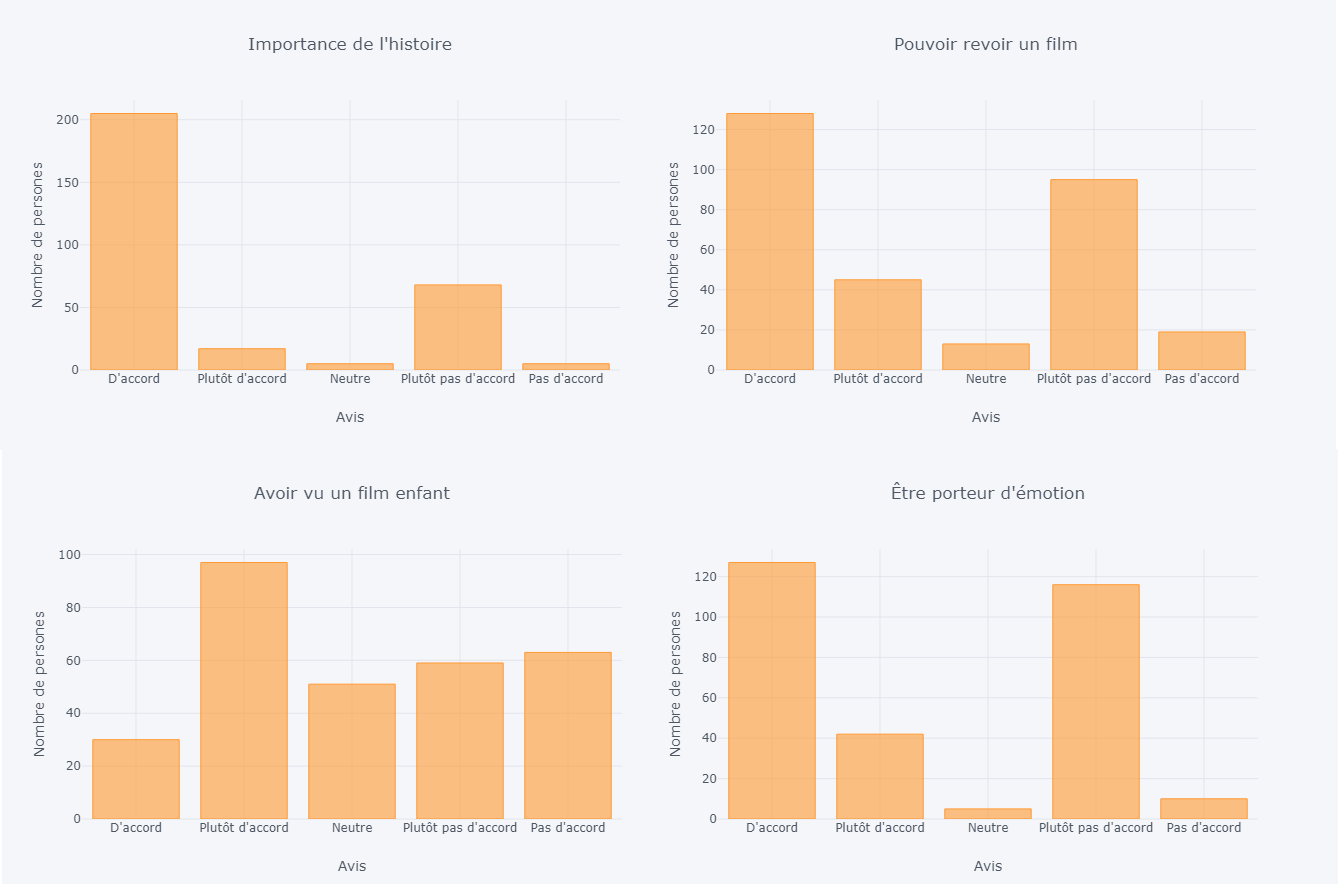
\includegraphics[keepaspectratio,scale=0.6]{h9.png}
	\caption{Proportion des caractéristique \#2}
\end{figure}~\\
Il s’agit ici de comparer les effectifs de chaque proportion pour chaque caractéristique. Il fallait donc récupérer le nombre d'occurrences de chaque jugement (d’accord, plutôt d’accord, neutre, plutôt pas d’accord, pas d’accord) avant de faire les tests statistiques. Les résultats obtenus sur le sondage sont visibles ci-dessus. 
\subsubsection{Application des tests}
Pour les tests statistiques nous avons toujours procédé de la même façon: vu qu’il faut comparer les effectifs de données catégorielles, nous avons fait deux séries de tests du $\chi^2$ :

\begin{wrapfigure}[12]{hbt}{5.5cm}
\begin{tabular}{|p{3cm}|p{2cm}|}
	\hline
	\rule{0cm}{5mm}
	Caractéristique & P-value obtenue \\
	\hline
	\rule{0cm}{5mm}
	Réplique & 7.934$e^{-68}$\\
	\hline
	\rule{0cm}{5mm}
	Musique & 1.397$e^{-12}$\\
	\hline
	\rule{0cm}{5mm}
	Histoire & 2.976$e^{-103}$\\
	\hline
	\rule{0cm}{5mm}
	Revoir le film & 7.303$e^{-35}$\\
	\hline
	\rule{0cm}{5mm}
	L’avoir vu enfant & 5.944$e^{-08}$\\
	\hline
	\rule{0cm}{5mm}
	Porteur d’émotion & 1.950$e^{-47}$ \\
	\hline
\end{tabular}
\end{wrapfigure}
~\\
\begin{itemize}
	\item La première série prend en compte tous les effectifs. Le test statistique permettra de confirmer ou non la présence d’un jugement dominant pour la caractéristique en question.
	\item La deuxième série est un test seulement sur les deux jugements ayant les plus grands effectifs. Si la p-value est inférieure à 5\%, cela voudra dire que de manière générale ce jugement pour cette caractéristique est majoritaire, et ce sans ambiguïté possible.
\end{itemize}
Les résultats obtenus pour la première série de test de $\chi^2$ sont visible ci-contre:
\alertsuccess{Nous pouvons donc infirmer toutes les hypothèses 9: il y a pour chaque caractéristique au moins une opinion dominante.}
\begin{wrapfigure}[15]{hbt}{5.5cm}
	\begin{tabular}{|p{3cm}|p{2cm}|}
		\hline
		\rule{0cm}{5mm}
		Caractéristique & P-value obtenue \\
		\hline
		\rule{0cm}{5mm}
		Réplique & 4.355$e^{-09}$\\
		\hline
		\rule{0cm}{5mm}
		Musique & 3.346$e^{-22}$\\
		\hline
		\rule{0cm}{5mm}
		Histoire & 1.117$e^{-16}$\\
		\hline
		\rule{0cm}{5mm}
		Revoir le film & 2.711$e^{-02}$\\
		\hline
		\rule{0cm}{5mm}
		L’avoir vu enfant & 7.189$e^{-03}$\\
		\hline
		\rule{0cm}{5mm}
		Porteur d’émotion & 0.4804 \\
		\hline
	\end{tabular}
\end{wrapfigure}
~\\
Les résultats obtenus pour la deuxième série de test de $\chi^2$ sont visibles ci-contre:\\
Ici nous pouvons remarquer que toute les tests révèlent une p-value <0.05 , excepté la p-value du "porteur d'émotion", qui elle est clairement au dessus (p-value = 0.48) du seuil. Nous pouvons donc affirmer :
\begin{itemize}
	\item Les répliques sont importantes pour qu'un film soit mémorable (D'accord)
	\item La musique est importante pour qu'un film soit mémorable (D'accord)
	\item La qualité de l'histoire est importante pour qu'un film soit mémorable (D'accord)
	\item Revoir un film est important pour qu'un film soit mémorable (D'accord)
	\item Avoir vu un film enfant est important pour qu'un film soit mémorable (D'accord)
	\item >L'hypothèse nulle est acceptée pour la caractéristique porteur d'émotion. On peut conclure que nous n'avons pas assez d'élément pour déterminer si oui ou non cette caractéristique est importante pour qu'un film soit mémorable
\end{itemize}
\alertsuccess{Nous pouvons donc confirmer toutes les hypothèse de la partie 9, exceptée pour être porteur d'émotion}
\subsection{Hypothèse 10}
H9 : Les étudiants de l’IMT reconnaissent plus facilement les films proposés.
\begin{itemize}
	\item $H_0 : \ \mu_{nonIMT} = \mu_{IMT}$
	\item $H_a : \ \mu_{nonIMT} \ne \mu_{IMT}$
\end{itemize}
Nous allons donc ici étudier les réponses des sondés en les divisant en deux population: étudiant de l’IMT ou non.
\subsubsection{Visualisation}
\begin{figure}[!h]
	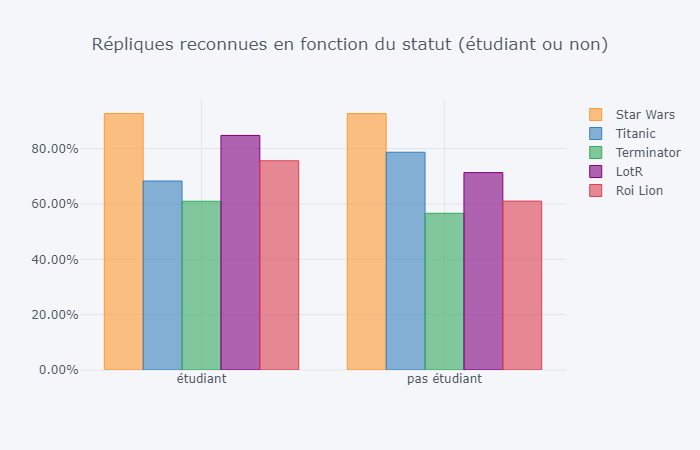
\includegraphics[keepaspectratio,scale=0.33]{h10.png}
	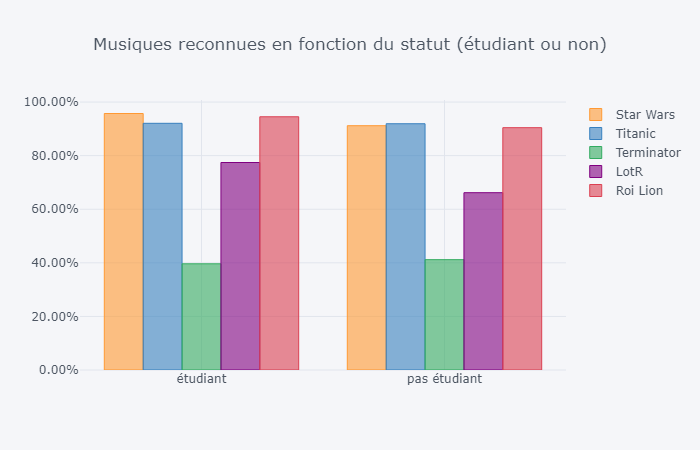
\includegraphics[keepaspectratio,scale=0.33]{h101.png}
	\caption{Répliques reconnues en fonction du statut (étudiant ou non)}
\end{figure}~\\

\subsubsection{ Application des test}
Nous appliquons ici le test de Student.
La moyenne de connaissance des films pour les étudiants IMT est de 0.75 et la moyenne de connaissance des films pour les non-étudiants IMT est de 0.7
136 personnes non IMT Atlantique ont répondu au sondage contre 164 étudiants IMT Atlantique. Les deux populations impliquées sont donc de proportions équivalentes.\\
Après application du test, nous obtenons les valeurs suivantes : $pvalue =   0.04971$, $t = 1.9704$.L'intervalle de confiance des différences de moyenne est de : [-0.10,0.00].\\
\alertsuccess{On remarque que l'hypothèse a une p-value inférieure à 0.05. Nous pouvons donc rejeter l'hypothèse nulle. Ainsi les étudiant d'IMT Atlantique ont plus tendance à reconnaître les films proposés comparé aux non-étudiants IMT Atlantique. }
En effet lors de la sélection des films, nous avions pensé qu'étant tous issus d'un milieu assez homogène, ce que nous pensions être connu l'était aussi pour les étudiants d'IMT Atlantique, mais peut être pas pour les autres. Ce test vient de le confirmer. 

\section{Analyse critique du sondage}
\subsection{Les critiques et biais du sondage:}
Le premier et plus important biais que nous avons noté lors de ce sondage est celui de la population des sondés. En effet, nous avons proposé ce sondage aux étudiants de l’IMT, au personnel de l’IMT ainsi qu’à nos familles respectives. Cependant, nous avons une population d’étudiants de l’IMT bien supérieure aux deux autres (plus de la moitié de la population sont des étudiants de l’IMT). Ainsi, mêmes si représentées, les différentes catégories d'âge et nationalité ont un poids bien inférieur.\\
Ensuite, le choix des 5 films est clairement biaisé. Nous sommes 6 dans notre groupe, 6 hommes français de 22-23 ans étudiants de l’IMT. Même si nous avons fait en sorte de choisir des “piliers” du cinéma d’époques et styles variés, nous étions conscients que notre objectivité était impossible. Nous nous attendions donc à avoir le plus de résultats positifs au blind test pour la catégorie à laquelle nous appartenons. Ceci se confirme lors de nos tests.\\
De même, avec les tests, nous nous sommes rendus compte que nous avions choisis un film trop connu (“Le roi lion”). Ainsi, ce film n’est pas du tout clivant (seulement 7\% des gens ne l’ont jamais vu). L’analyse qui en découle ne représente pas fidèlement la réalité.\\
De plus, nous avons remarqué un biais non négligeable lors du blind test. En effet, notre blind test est constitué autour de 5 films, avec pour chacun une réplique et une musique. Mettons-nous alors en situation de blind test. Une réplique que vous connaissez vient d’apparaître. Après un moment de réflexion, le nom du film vous revient et vous l’indiquez. Votre mémoire à court terme se met en marche et le nom de ce film reste dans un coin de votre tête. Ensuite, une fois arrivé à la musique de ce même film, vous vous en rappelez beaucoup plus facilement parce que vous vous l’êtes remémoré juste avant. Cependant, dans la situation où la musique passe en premier, peut-être n’auriez vous pas retrouvé le nom du film. Ainsi, l'association musique/réplique est un biais en soi. Cependant, ce biais est inévitable, étant donné le sujet de notre sondage.\\
Après, notre question préliminaire “Pensez-vous reconnaitre plus un film par sa musique ou par ses répliques?” que nous avons formulé a provoqué un biais que nous avons remarqué lors des tests. En effet, un certain nombre de personnes reconnaissent aussi bien la musique que la réplique, alors que notre question ne permet qu’un choix de l’un ou l’autre. Lors des tests, nous avons donc remarqué qu’un bon nombres de nos résultats étaient légèrement faussés par ces personnes qui ont bien répondu aux répliques et musiques du blind test. Cependant, nous l’avons décidé en connaissance de cause, pour vraiment confronter les deux propositions. Nous craignions qu’un choix “répliques et musiques” aurait poussé tous les participants à cliquer dessus par facilité.\\
De plus, le sondage étant en ligne et envoyé par mail aux sondés, nous ne pouvons prévenir d’éventuelles “tricheries”. En effet, les sondés ont accès internet sur leurs ordinateurs au moment du sondage. Ils peuvent également être en présence d’autres personnes lors du remplissage, ce qui peut biaiser les données récoltées.\\

\subsection{Les solutions qui pourraient être trouvées pour pallier aux biais}
Par manque de temps et de moyens, nous n’avons pas échantillonné notre population sondée. Nous aurions pu faire un échantillonnage stratifié auprès d’une très large population en utilisant d’autres moyens de diffusion de sondage pour pouvoir vérifier le fait qu’un film soit “culte” pour le plus de types de personnes possibles. Nous aurions pris comme caractéristiques principales l’âge et la nationalité des personnes pour piocher nos différents sous-échantillons. Cet échantillonnage irait pallier notre biais le plus important, à savoir la grande proportion d’étudiant de l’IMT dans notre sondage. En prenant un plus large échantillon pour le sondage idéal, nous aurions moins de problèmes avec la population qui ne connaît pas Le Roi Lion puisqu'elle sera sûrement plus grande, et donc, plus représentative de la réalité et apte à être analysée.\\
Afin de choisir les films à tester le plus efficacement possible, il faudrait recueillir des données sur une première population (plus petite) et réaliser un pré-sondage pour demander quels films sont cultes par leurs musiques et par leurs répliques afin de choisir les plus récurrents.\\
Pour le biais de la mémoire à court terme des sondés, une solution serait d’augmenter le nombre de films cultes pour noyer les sondés d’informations. Toutefois, le sondage gagnerait en longueur et pourrait être trop long pour les sondés. Il serait aussi possible de de séparer les répliques des films des musiques de films. On ne peut donc plus vérifier qu’un film est culte s’il est deviné par blind test et réplique. Une autre solution serait de prendre des films moins connus. Nous aurions alors plus d’informations sur la différence réplique/musique pour définir un film culte, mais le but de notre sondage perdrait en sens puisqu’on ne testerait plus les caractéristiques de films vraiment cultes.\\
De plus, en réalisant le sondage directement auprès des sondés, en face à face, nous pourrions empêcher tout problème de “tricherie”. Cependant, le volume horaire engendré, pour atteindre un échantillon identique, serait beaucoup trop important et impossible pour le délai de ce projet.
\section{Remarques}
Plusieurs retours de la part des sondés ont été très positifs du fait qu’ils ont aimé participer à ce sondage et nous l’ont signalé, en particulier à cause du blind test. Plusieurs personnes nous ont aussi fait part de leur intérêt quant à nos résultats ou cherchaient à savoir quelle était la musique - réplique qu’ils n’avaient pas reconnus.\\
Cet attrait du sondage se retrouve dans nos résultats puisque plus de 300 personnes ont correctement complété ce sondage et seulement 80 personnes ont abandonné en cours de remplissage pour ce long sondage qui durait presque 8 minutes. De plus, nous estimons qu’une bonne part de ces abandons sont dus à la contrainte de devoir écouter l’audio, ce qui ne peut pas être fait dans n’importe quel contexte.\\

\newpage
\section{Annexes}
\subsection{Retrouver l'ensemble des résultat}
L'ensemble des tests statistiques ont été fait sur un Jupyter Notebook disponible sur le lien github suivant (fichier nommé : Projet Stats.ipynb). Si vous n'avez pas installé Jupyter Notebook, vous pouvez télécharger le fichier HTML (Projet Stats.ipynb). Les graphiques ne sont pas visibles dans le mode aperçu de github.
\alertinfo{\url{https://github.com/Syndorik/ProjetStats}. Il faut télécharger le fichier afin de pouvoir visualiser les graphiques}

\subsection{Remerciement}
\begin{itemize}
	\item Ce rapport a été fait sous LaTeX. Nous remercions \textbf{Armand FOUCAULT} et \textbf{Benoît PORTEBOEUF} pour avoir créer le template IMT Atlantique sur LaTeX. Il est disponible sur le lien suivant :
	\alertinfo{https://github.com/bporteboeuf/imtaLatexTemplate}
	\item Nous remercions toue les personnes pour avoir répondu au sondage
\end{itemize}


\imtaMakeCover

\end{document}
%%%%%%%%%% END %%%%%%%%%% 
%%%%%%%%%%%%%%%%%%%%%%%%% 
